
\documentclass{article}
\usepackage[utf8]{inputenc}
\usepackage{amsmath}
\usepackage{tcolorbox}
\tcbuselibrary{theorems}

\begin{document}

\begin{tcolorbox}[colback=blue!5!white,colframe=blue!75!black,title=Question 1]
A rectangular region of land is divided into 54 square lots of equal area \( S \) in square units. The length of the region is 1.5 times the width of the region. If the width of the region is \( a\sqrt{S} \) units, what is the value of \( a \)?

\begin{itemize}
    \item[A.] 5
    \item[B.] 6
    \item[C.] 7
    \item[D.] 8
\end{itemize}
\end{tcolorbox}

\begin{tcolorbox}[colback=green!10, colframe=green!50!black,title=Answer to Question 1]
\textbf{Correct Answer: B}  
\end{tcolorbox}




\vspace{20pt}

\begin{tcolorbox}[colback=blue!5!white,colframe=blue!75!black,title=Question 2]
In the given pair of equations, \( a \) and \( b \) are constants. The graph of this pair of equations in the xy-plane is a pair of perpendicular lines. Which of the following pairs of equations also represents a pair of perpendicular lines?

\[
5x + 7y = 1
\]
\[
ax + by = 1
\]

\begin{itemize}
    \item[A.] \( 10x + 7y = 1, \quad ax - 2by = 1 \)
    \item[B.] \( 10x + 7y = 1, \quad ax + 2by = 1 \)
    \item[C.] \( 10x + 7y = 1, \quad 2ax + by = 1 \)
    \item[D.] \( 5x - 7y = 1, \quad ax + by = 1 \)
\end{itemize}
\end{tcolorbox}

\begin{tcolorbox}[colback=green!10, colframe=green!50!black,title=Answer to Question 2]
\textbf{Correct Answer: B}  
\end{tcolorbox}

\vspace{20pt}

\begin{tcolorbox}[colback=blue!5!white,colframe=blue!75!black,title=Question 3]
A real estate company offers a series of three webinars. 2,000 people attended the first webinar. 65\% of the people who attended the first webinar attended the second webinar, and 44\% of the people who attended both the first and second webinars attended the third webinar. 

If those who attended the first but did not attend the second webinar, 31\% attended the third webinar. How many people attended both the first and third webinars but did not attend the second webinar?

\end{tcolorbox}

\begin{tcolorbox}[colback=green!10, colframe=green!50!black,title=Answer to Question 3]
\textbf{Correct Answer: 217}  
\end{tcolorbox}

\vspace{20pt}

\begin{tcolorbox}[colback=blue!5!white,colframe=blue!75!black,title=Question 4]
The functions \( f \) and \( g \) are defined by the given equations, where \( x \geq 0 \). 

\[
f(x) = 19(1.27)^x + 43
\]
\[
g(x) = 8(0.77)^x
\]

Which of the following equations displays, as a constant or coefficient, the maximum value of the function it defines, where \( x \geq 0 \)?

\begin{itemize}
    \item[A.] I only
    \item[B.] II only
    \item[C.] I and II
    \item[D.] Neither I nor II
\end{itemize}
\end{tcolorbox}

\begin{tcolorbox}[colback=green!10, colframe=green!50!black,title=Answer to Question 4]
\textbf{Correct Answer: B}  
\end{tcolorbox}




\begin{tcolorbox}[colback=blue!5!white,colframe=blue!75!black,title=Question 5]
Circle \( F \) in the xy-plane is represented by the equation:
\[
(x - 13)^2 + (y - 9)^2 = 196
\]
Circle \( G \) is obtained by shifting circle \( F \) 5 units to the left and 11 units up.

An equation representing circle \( G \) is:
\[
(x + h)^2 + (y + k)^2 = 196
\]
where \( h \) and \( k \) are constants.

What is the value of \( h + k \)?
\end{tcolorbox}

\begin{tcolorbox}[colback=green!10, colframe=green!50!black,title=Answer to Question 5]
\textbf{Correct Answer: -28}  
\end{tcolorbox}

\vspace{20pt}

\begin{tcolorbox}[colback=blue!5!white,colframe=blue!75!black,title=Question 6]
The function \( q \) is defined by:
\[
q(x) = a |x - 9|^2 - 87 |x - 9| + b
\]
where \( a \) and \( b \) are constants, and \( a > b > 87 \).

If \( q(639) = h \) and \( q(-621) = k \), where \( h \) and \( k \) are constants, what is the value of:
\[
9(-639)^{h-k} + 621(9)^{k-h}?
\]
\end{tcolorbox}

\begin{tcolorbox}[colback=green!10, colframe=green!50!black,title=Answer to Question 6]
\textbf{Correct Answer: 630}  
\end{tcolorbox}

\vspace{20pt}

\begin{tcolorbox}[colback=blue!5!white,colframe=blue!75!black,title=Question 7]
In the given equation, \( a \) and \( b \) are positive constants. A solution to the equation is \( x = 42 \).

\[
x(9x - 2a) + b(9x - 2a) - (x + b) = 0
\]

What is the value of \( a \)?
\end{tcolorbox}

\begin{tcolorbox}[colback=green!10, colframe=green!50!black,title=Answer to Question 7]
\textbf{Correct Answer: 188.5 }  
\end{tcolorbox}

\vspace{20pt}

\begin{tcolorbox}[colback=blue!5!white,colframe=blue!75!black,title=Question 8]
A right rectangular prism has a base area of \( 28p \) square centimeters (\(\text{cm}^2\)). The length of the base of the rectangular prism is 12 cm, and the height of the rectangular prism is 4 cm.

Which expression represents the surface area, in \(\text{cm}^2\), of the right rectangular prism?

\begin{itemize}
    \item[A.] \( \frac{512p}{3} \)
    \item[B.] \( \frac{224p}{3} + 96 \)
    \item[C.] \( 56p + 192 \)
    \item[D.] \( 560p + 96 \)
\end{itemize}
\end{tcolorbox}

\begin{tcolorbox}[colback=green!10, colframe=green!50!black,title=Answer to Question 8]
\textbf{Correct Answer: B}  
\end{tcolorbox}



\begin{tcolorbox}[colback=blue!5!white,colframe=blue!75!black,title=Question 9]
The expression 
\[
\frac{x^{-2} y^{\frac{1}{2}}}{x^{\frac{1}{3}} y^{-1}}
\]
where \( x > 1 \) and \( y > 1 \), is equivalent to which of the following?

\begin{itemize}
    \item[A.] \( \frac{\sqrt{y}}{\sqrt[3]{x^2}} \)
    \item[B.] \( \frac{y \sqrt{y}}{\sqrt[3]{x^2}} \)
    \item[C.] \( \frac{y \sqrt{y}}{x \sqrt{x}} \)
    \item[D.] \( \frac{y \sqrt{y}}{x^2 \sqrt[3]{x}} \)
\end{itemize}
\end{tcolorbox}

\begin{tcolorbox}[colback=green!10, colframe=green!50!black,title=Answer to Question 9]
\textbf{Correct Answer: D}  
\end{tcolorbox}

\newpage

\begin{tcolorbox}[colback=blue!5!white,colframe=blue!75!black,title=Question 10]
The function \( z \) is defined by the equation:
\[
z(w) = (0.829)^{2w}
\]
The value of \( z(w) \) decreases by \( p\% \) for each increase by 1 in the value of \( w \). Which of the following is closest to the value of \( p \)?

\begin{itemize}
    \item[A.] 0.171
    \item[B.] 0.829
    \item[C.] 17.1
    \item[D.] 31.3
\end{itemize}
\end{tcolorbox}

\begin{tcolorbox}[colback=green!10, colframe=green!50!black,title=Answer to Question 10]
\textbf{Correct Answer: D}  
\end{tcolorbox}

\vspace{20pt}

\begin{tcolorbox}[colback=blue!5!white,colframe=blue!75!black,title=Question 11]
\[
-16(5x - 3)^2 + 4(5x - 2)^2
\]

The given expression can be rewritten as:
\[
\frac{a}{4} x^2 + \frac{b}{4} x + \frac{c}{4}
\]
where \( a, b, c \) are constants. What is the value of \( a + b + c \)?



\begin{itemize}
    \item[A.] -112
    \item[B.] -56
    \item[C.] -28
    \item[D.] -7
\end{itemize}
\end{tcolorbox}

\begin{tcolorbox}[colback=green!10, colframe=green!50!black,title=Answer to Question 11]
\textbf{Correct Answer: A}  
\end{tcolorbox}



\begin{tcolorbox}[colback=blue!5!white,colframe=blue!75!black,title=Question 12]
The graph of line \( h \) is shown in the xy-plane. Line \( k \) (not shown) is defined by the equation:

\[
sx + 40y = t
\]

where \( s \) and \( t \) are constants. If line \( k \) is graphed in this xy-plane, the result is a graph of two linear equations. This system of two linear equations has no solution.

Which of the following is \textbf{NOT} a possible value of \( t \)?



\begin{itemize}
    \item[A.] -360
    \item[B.] -9
    \item[C.] 72
    \item[D.] 200
\end{itemize}


\begin{center}
    

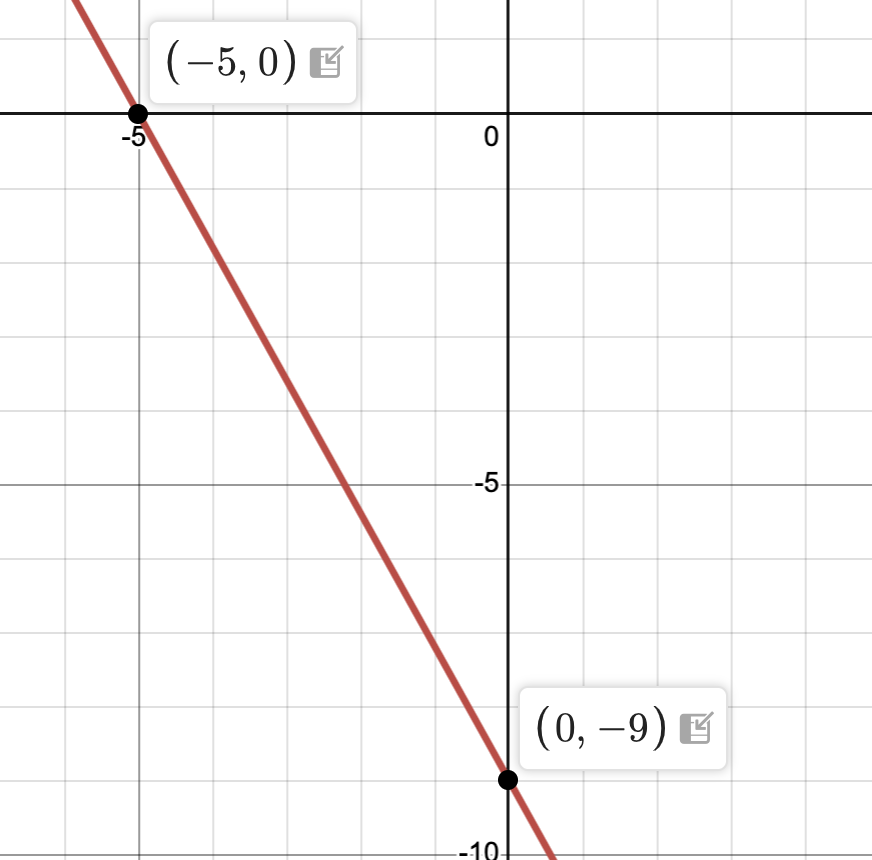
\includegraphics[width=0.6\linewidth]{f4.png}
\end{center}
\end{tcolorbox}

\begin{tcolorbox}[colback=green!10, colframe=green!50!black,title=Answer to Question 12]
\textbf{Correct Answer: A}  
\end{tcolorbox}



\end{document}